\section{Drone Navigation}

\subsection{Functional Requirements}

	\begin{flushleft}
		\begin{itemize}
			\item{\textbf{R1:}} FMDS will \textbf{follow} the ranger
		  		\begin{itemize}
		  			\item{\textbf{R1.1}} FMDS will allow the ranger to perform \textbf{initialisation} for the drone.
		  				\begin{itemize}
		  					\item{\textbf{R1.1.1}} FMDS will allow the ranger to set himself as the validated object.
		  						\begin{itemize}
									\item The validated object will not be treated as a normal object when searching the field of view of the drone. Notifications are sent to the ranger when objects are detected, however notifications will not be sent every time the ranger is identified.
								\end{itemize}
		  					\item{\textbf{R1.1.2}} FMDS will allow the ranger to initialise his beacon.
								\begin{itemize}
									\item The beacon will allow the drone to know where the ranger is at any moment in time, which will assist in expanding the drone's field of view since the drone will not need to be facing the ranger.
								\end{itemize}
		  				\end{itemize}

		  			\item{\textbf{R1.2}} FMDS will allow the ranger to specify a \textbf{flight pattern} for the drone
		  				\begin{itemize}
		  					\item{\textbf{R1.2.1}} FMDS will detect objects while on its flight path.
								\begin{itemize}
									\item Object recognition (as a service) will be running from the moment the ranger initialises the drone until the moment it lands. Rectangles will be drawn around identified objects along with the label for each identified object.
								\end{itemize}
		  					\item{\textbf{R1.2.2}} FMDS will record live video while on its flight path.
								\begin{itemize}
									\item Stored video data will be used as further training data for the object recognition model.
								\end{itemize}
						  \end{itemize}
			\end{itemize}
		\end{itemize}

		\begin{itemize}
			\item{\textbf{R2:}} FMDS will \textbf{patrol} the area around the ranger
				\begin{itemize}
					\item{\textbf{R2.1}} FMDS will patrol by flying in the designated \textbf{flight pattern} around the ranger.
						\begin{itemize}
							\item The desired flight pattern will be chosen upon initialisation and will remain as the default flight pattern unless updated during the drone's flight.
						\end{itemize}
					\item{\textbf{R2.2}} FMDS will perform \textbf{object detection}.
						\begin{itemize}
							\item{\textbf{R2.2.1}} FMDS will drop a pin of the object detected on the 2D map.
								\begin{itemize}
									\item The coordinates of the drone's current location will be sent to the server with a command to drop a pin at that location. In addition to the coordinates, the object's classification (elephant, rhino, person, etc) will will be sent to the server. the server will then attempt to assess the identified object's threat level. The server will then send an update to the ranger's app on their phone which will generate a pin. The pin will be coloured based on the perceived threat level. 
								\end{itemize} 
						\end{itemize}
					\item{\textbf{R2.3}} FMDS will \textbf{record} video footage during its surveillance.
						\begin{itemize}
							\item Stored video data will be used as further training data for the object recognition model.
						\end{itemize} 
					\item{\textbf{R2.4}} FMDS will take \textbf{snapshots} of the reserve during its surveillance.
						\begin{itemize}
							\item{\textbf{R2.4.1}} FMDS will build a 2D map of the reserve.
								\begin{itemize}
									\item Snapshots will be periodically taken and stitched together at a later stage to create a virtual 2D map which is regularly updated. The updated 2D map will be useful to the rangers when wildlife, plantlife and the general health of the reserve is monitored.
								\end{itemize} 
						\end{itemize}
				\end{itemize}
		\end{itemize}
	\end{flushleft}

\subsection{Use Case Diagram}
\begin{center}
	\begin{flushleft}
		\begin{figure}[h!]
			\centering
			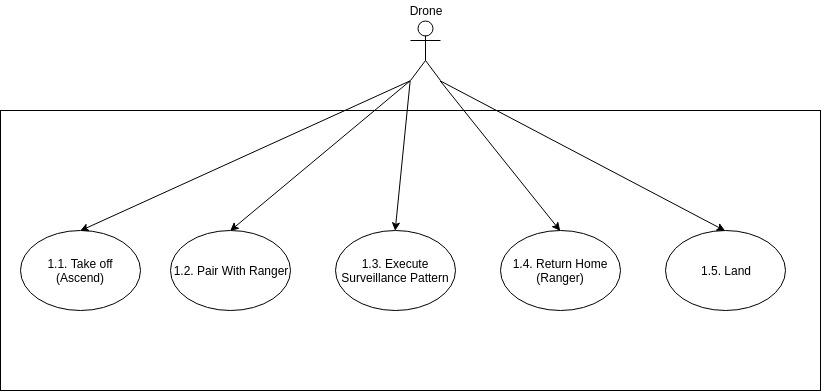
\includegraphics[scale=0.5]{./assets/images/navigation-ucd.jpg}
			\label{fig: object-recognition-ucd }
			\caption{Drone Navigation Use Case Diagram}
		\end{figure}

	\end{flushleft}
\end{center}

\subsection{Technical Requirements}
	\begin{flushleft}
		\begin{itemize}
				\item Python v2.7 
		\end{itemize}
	\end{flushleft}
